% 2010 年湖南卷文科第 18 题：长方体 ABCD-A1B1C1D1，M 为棱 CC1 的中点。
% 来源 PDF：普通高考/2010/2010湖南文.pdf，SHA-256 38611c33c9da2139ad6cd4117513ee144b09a6860180eb976c446b4858ada122。
% 原页：第 2 页（A3 三栏）第 1 栏上部，书页码 604。
% 重绘依据：照原页斜二测画法，前面 BB1C1C，后面 AA1D1D 向右上平移；
%   实线为可见棱，虚线为被遮挡的三条棱 AA1、AB、AD；
%   另以实线画出 B1M 与 BM（题中两个平面的交线所在的两条线段）。
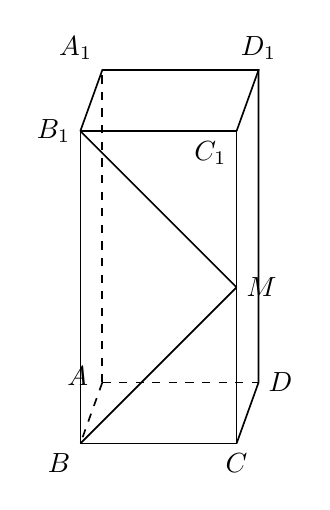
\begin{tikzpicture}[scale=0.62, semithick]
  \coordinate (B)  at (0,0);
  \coordinate (C)  at (3.2,0);
  \coordinate (C1) at (3.2,6.4);
  \coordinate (B1) at (0,6.4);
  \coordinate (A)  at (0.45,1.25);
  \coordinate (D)  at (3.65,1.25);
  \coordinate (A1) at (0.45,7.65);
  \coordinate (D1) at (3.65,7.65);
  \coordinate (M)  at (3.2,3.2);

  % 可见棱
  \draw (B) -- (C) -- (C1) -- (B1) -- cycle;
  \draw (B1) -- (A1) -- (D1) -- (C1);
  \draw (D1) -- (D) -- (C);

  % 被遮挡的棱
  \draw[dashed] (A) -- (B);
  \draw[dashed] (A) -- (D);
  \draw[dashed] (A) -- (A1);

  % 辅助线段：B1M 与 BM
  \draw (B1) -- (M);
  \draw (B) -- (M);

  \node[below left]  at (B)  {$B$};
  \node[below]       at (C)  {$C$};
  \node[left]        at (B1) {$B_1$};
  \node[below left]  at (C1) {$C_1$};
  \node[above left]  at (A1) {$A_1$};
  \node[above]       at (D1) {$D_1$};
  \node[left, xshift=-1.5pt, yshift=2.5pt]  at (A)  {$A$};
  \node[right]       at (D)  {$D$};
  \node[right]       at (M)  {$M$};
\end{tikzpicture}
